%% ----------------------------------------------------------------
%% Thesis.tex -- MAIN FILE (the one that you compile with LaTeX)
%% ---------------------------------------------------------------- 

% Set up the document
\documentclass[a4paper, 11pt, oneside]{Thesis}  % Use the "Thesis" style, based on the ECS Thesis style by Steve Gunn
\graphicspath{Figures/}  % Location of the graphics files (set up for graphics to be in PDF format)

% Include any extra LaTeX packages required
\usepackage[square, numbers, comma, sort&compress]{natbib}  % Use the "Natbib" style for the references in the Bibliography
\usepackage{verbatim}  % Needed for the "comment" environment to make LaTeX comments
\usepackage{vector}  % Allows "\bvec{}" and "\buvec{}" for "blackboard" style bold vectors in maths
\usepackage{amsmath,amssymb,amsopn,amstext,amsfonts}
\hypersetup{urlcolor=blue, colorlinks=true}  % Colours hyperlinks in blue, but this can be distracting if there are many links.

%% ----------------------------------------------------------------
\begin{document}
	\frontmatter      % Begin Roman style (i, ii, iii, iv...) page numbering
	
	% Set up the Title Page
	\title  {Study of Efficient Mixed-Integer Planning for Autonomous Vehicles in Densely Cluttered Environments}
	\authors  {\texorpdfstring
		{{Mosam Sanjay Dabhi}}
		{Mosam Sanjay Dabhi}
	}
	\addresses  {\groupname\\\deptname\\\univname}  % Do not change this here, instead these must be set in the "Thesis.cls" file, please look through it instead
	\date       {\today}
	\subject    {}
	\keywords   {}
	
	\maketitle
	%% ----------------------------------------------------------------
	
	\setstretch{1.3}  % It is better to have smaller font and larger line spacing than the other way round
	
	% Define the page headers using the FancyHdr package and set up for one-sided printing
	\fancyhead{}  % Clears all page headers and footers
	\rhead{\thepage}  % Sets the right side header to show the page number
	\lhead{}  % Clears the left side page header
	
	\pagestyle{fancy}  % Finally, use the "fancy" page style to implement the FancyHdr headers
	
	%% ----------------------------------------------------------------
	% Declaration Page required for the Thesis, your institution may give you a different text to place here
	\Declaration{
		
		\addtocontents{toc}{\vspace{1em}}  % Add a gap in the Contents, for aesthetics
		
		I, Mosam Sanjay Dabhi, declare that this thesis titled, `Study of Efficient Mixed-Integer Planning for Autonomous Vehicles in Densely Cluttered Environments' and the work presented in it are my own. I confirm that:
		
		\begin{itemize} 
			\item[\tiny{$\blacksquare$}] This work was done wholly or mainly while in candidature for a research degree at this University.
			
			\item[\tiny{$\blacksquare$}] Where any part of this thesis has previously been submitted for a degree or any other qualification at this University or any other institution, this has been clearly stated.
			
			\item[\tiny{$\blacksquare$}] Where I have consulted the published work of others, this is always clearly attributed.
			
			\item[\tiny{$\blacksquare$}] Where I have quoted from the work of others, the source is always given. With the exception of such quotations, this thesis is entirely my own work.
			
			\item[\tiny{$\blacksquare$}] I have acknowledged all main sources of help.
			
			\item[\tiny{$\blacksquare$}] Where the thesis is based on work done by myself jointly with others, I have made clear exactly what was done by others and what I have contributed myself.
			\\
		\end{itemize}
		
		
		Signed:\\
		\rule[1em]{25em}{0.5pt}  % This prints a line for the signature
		
		Date:\\
		\rule[1em]{25em}{0.5pt}  % This prints a line to write the date
	}
	\clearpage  % Declaration ended, now start a new page
	
	%% ----------------------------------------------------------------
	% The "Funny Quote Page"
	\pagestyle{empty}  % No headers or footers for the following pages
	
	\null\vfill
	% Now comes the "Funny Quote", written in italics
	\textit{``When Larry and Sergey founded Google Search, one of the things that struck me is that it was available for everyone to use. We deeply desire our services to work for everyone. And that inherently means we have to work with partners. That is the thesis underlying everything we do.''}
	
	\begin{flushright}
		Sundar Pichai
	\end{flushright}
	
	\vfill\vfill\vfill\vfill\vfill\vfill\null
	\clearpage  % Funny Quote page ended, start a new page
	%% ----------------------------------------------------------------
	
	% The Abstract Page
	\addtotoc{Abstract}  % Add the "Abstract" page entry to the Contents
	\abstract{
		\addtocontents{toc}{\vspace{1em}}  % Add a gap in the Contents, for aesthetics
		
		In this work, we study the problem of planning
		safe and dynamically feasible trajectories through a densely cluttered environment. We devise an experimental approach to the design of
		smooth trajectories for quadrotor unmanned aerial vehicles
		(UAVs), which are free of collisions with obstacles along their
		entire length. To avoid the non-convex constraints normally
		required for obstacle-avoidance, we perform a mixed-integer
		optimization in which polynomial trajectories are assigned to
		convex regions which are known to be obstacle-free. Prior
		approaches have used the faces of the obstacles themselves to
		define these convex regions. The innovative approach brought about here is the use of Iterative Regional Inflation by Semidefinite Programming(IRIS)
		algorithm, a recently developed technique for greedy convex segmentation~\cite{deits2015computing}, to pre-compute convex regions of safe space. The aforementioned approach results in a substantially reduced number of integer variables, which improves the speed with which the optimization can be solved to its global optimum, even for tens or hundreds of obstacle faces. In addition, prior approaches have typically enforced obstacle avoidance at a finite set of sample or knot points. This study supports a technique based on sums-of-squares (SOS) programming that allows the user to ensure that the entire piecewise polynomial trajectory is free of collisions using convex constraints. To support this study, we demonstrate this technique in 2D and in 3D random environments and also in a cluttered indoor environment given by a dense pointcloud.
		
	}
	
	\clearpage  % Abstract ended, start a new page
	%% ----------------------------------------------------------------
	
	\setstretch{1.3}  % Reset the line-spacing to 1.3 for body text (if it has changed)
	
	% The Acknowledgements page, for thanking everyone
	\acknowledgements{
		\addtocontents{toc}{\vspace{1em}}  % Add a gap in the Contents, for aesthetics
		
		I acknowledge my department, 'Electronics and Communication Engineering Department' of S.V.N.I.T. for throughly supporting my work and I thank especially my seminar report advisor, 'Dr. J. N. Sarvaiya' for his valuable inputs and suggestions without which this report would not have been possible.
		
	}
	\clearpage  % End of the Acknowledgements
	%% ----------------------------------------------------------------
	
	\pagestyle{fancy}  %The page style headers have been "empty" all this time, now use the "fancy" headers as defined before to bring them back
	
	
	%% ----------------------------------------------------------------
	%\lhead{\emph{Contents}}  % Set the left side page header to "Contents"
	\tableofcontents  % Write out the Table of Contents
	
	%% ----------------------------------------------------------------
	%\lhead{\emph{List of Figures}}  % Set the left side page header to "List if Figures"
	\listoffigures  % Write out the List of Figures
	
	%% ----------------------------------------------------------------
	%\lhead{\emph{List of Tables}}  % Set the left side page header to "List of Tables"
	\listoftables  % Write out the List of Tables
	
	%% ----------------------------------------------------------------
	\setstretch{1.5}  % Set the line spacing to 1.5, this makes the following tables easier to read
	\clearpage  % Start a new page
	%\lhead{\emph{Abbreviations}}  % Set the left side page header to "Abbreviations"
	%\listofsymbols{ll}  % Include a list of Abbreviations (a table of two columns)
	%{
	% \textbf{Acronym} & \textbf{W}hat (it) \textbf{S}tands \textbf{F}or \\
	%\textbf{LAH} & \textbf{L}ist \textbf{A}bbreviations \textbf{H}ere \\
	
	%}
	
	%% ----------------------------------------------------------------
	\clearpage  % Start a new page
	%\lhead{\emph{Physical Constants}}  % Set the left side page header to "Physical Constants"
	%\listofconstants{lrcl}  % Include a list of Physical Constants (a four column table)
	%{
	% Constant Name & Symbol & = & Constant Value (with units) \\
	%Speed of Light & $c$ & $=$ & $2.997\ 924\ 58\times10^{8}\ \mbox{ms}^{-\mbox{s}}$ (exact)\\
	
	%}
	
	%% ----------------------------------------------------------------
	
	%\lhead{\emph{Symbols}}  % Set the left side page header to "Symbols"
	%\listofnomenclature{lll}  % Include a list of Symbols (a three column table)
	%{
	% symbol & name & unit \\
	%$a$ & distance & m \\
	%$P$ & power & W (Js$^{-1}$) \\
	%& & \\ % Gap to separate the Roman symbols from the Greek
	%$\omega$ & angular frequency & rads$^{-1}$ \\
	%}
	%% ----------------------------------------------------------------
	% End of the pre-able, contents and lists of things
	% Begin the Dedication page
	
	\setstretch{1.5}  % Return the line spacing back to 1.3
	
	\pagestyle{empty}  % Page style needs to be empty for this page
	%\dedicatory{For/Dedicated to/To my\ldots}
	
	\addtocontents{toc}{\vspace{2em}}  % Add a gap in the Contents, for aesthetics
	
	
	%% ----------------------------------------------------------------
	\mainmatter	  % Begin normal, numeric (1,2,3...) page numbering
	\pagestyle{fancy}  % Return the page headers back to the "fancy" style
	
	% Include the chapters of the thesis, as separate files
	% Just uncomment the lines as you write the chapters
	
	\chapter{Introduction}




\section{Background motivation and need for this survey study}


For autonomous vehicles traversing in real world environments, robust obstacle avoidance is a fundamental safety requirement. However, ensuring obstacle avoidance is complicated. We therefore wish to compute safe and optimal trajectories with respect to a cluttered environment. However, computing optimal trajectories through cluttered environments introduces additional computational complexity as the number of obstacles considered in the optimization increases. Advances in research have brought the quadrotor to a level of sophistication that is making it increasingly attractive
for a variety of commercial applications like surveying and delivery. In order for these applications to become a reality, we now need algorithms that can deal reliably with environments that are substantially more cluttered than a laboratory setting. The most successful algorithms put forward to enable quadrotors to avoid obstacles often require an exponential
increase in planning time with respect to the number of obstacles by, for example, introducing an integer variable for each face of obstacles in the environment. Most of these algorithms therefore start to perform poorly as the number of obstacles is increased beyond a modest handful of them.~\cite{mellinger2012mixed,schouwenaars2001mixed}.

For planning trajectories with obstacle avoidance in a
known environment, generally we used to add non-convex
constraints to an optimization for obstacle avoidance in order
to ensure that our trajectory remains outside the set of ob-
stacles. Such constraints prevent us from finding guarantees
of completeness or global optimality in our program. We
can avoid some of the problems of non-convex constraints
by adding a discrete component to optimization. So for that,
if we model the non-convex set of obstacle-free states as
union of finitely many convex regions, then we can perform
a mixed-integer convex optimization in which the integer
variables correspond to assignment of trajectory segments to
convex regions. But, the approach mentioned is not without
consequences, as even the addition of binary variables (con-
strained to either take values 0 or 1) makes the problem from
linear program into mixed-integer linear program, which is
known to be NP-complete (as it is both NP and NP-hard).
Earlier implementations typically used the faces of each
obstacle to define the convex safe regions, which was used
to encode obstacle avoidance for UAVs as a mixed integer
linear program (MILP) by~\cite{schouwenaars2001mixed,culligan2006online,hao2005differential,richardsco}.

Recently, it has been suggested that the challenges of
increasing obstacle density may be overcome by the novel
Iterative Regional Inflation by semidifinite programming
algorithm (IRIS) that segments space into obstacle-free
regions. Planning paths through this segmentation can be
accomplished using mixed-integer convex optimization, with
the complexity growing with the much more manageable
number of free-space segments instead of the number of
obstacle faces. Hence, it can produce trajectories in environ-
ments containing many more obstacles than was previously
demonstrated. Moreover the non-penetration constraint that
the algorithm enforces along the entire path promise better
performance with small obstacles than previous approaches
that rely on sampling. We hypothesized that it would be
possible to aggressively fly a small quadrotor through en-
vironments containing greater number of obstacles than
ever demonstrated before by leveraging IRIS, MISDPs, and model-based control approaches. This document presents experimental validation of this hypothesis and of the planning algorithm introduced in~\cite{deits2015efficient}. 

\section{Related Work}

A few planning algorithms have been successfully applied to planning for quadrotors in moderately crowded environments. The approach in~\cite{richter2013polynomial} consisted of running RRT* in the
entire space where the quadrotor might fly. The algorithm
only expanded the randomly-exploring tree with straight
paths in order to make its expansion more efficient. It there-
fore resulted in a piece-wise linear collision-free trajectory.
Finally, the algorithm computed a smooth trajectory using a
quadratic program between each node along the path returned
by RRT*. Although a very efficient approach, relying on
sampling of space in order to check for collisions makes it
potentially difficult to deal with very small obstacles like
the strings used in our experiment. ~\cite{mellinger2012mixed} demonstrated the use of mixed-integer quadratic programs in order to plan collision-free trajectories. In this particular work, the integer
variable enforced non-penetration by making sure that the
sampled location is on the collision-free side of at least one
of the faces of each obstacle. The approach worked well in
practice, but it suffered from having the number of integer
variables grow rapidly with the number of obstacles. The
technique once again cannot guarantee to generate collision-
free trajectories between sample points, unlike our presented
approach.

IRIS, the described choice of algorithm for convex segmentation
of free-space, has previously been used in the context of
collision-free footstep planning~\cite{deits2014convex}. In this application, the algorithm generated obstacle-free regions in the robot’s configuration space. A mixed-integer program was then used to assign steps to each regions while simultaneously optimizing the pose of the robot. ~\cite{deits2015efficient} then went on to demonstrate that
we could formulate the problem of planning minimum-snap
collision-free trajectories as a mixed-integer semidefinite
program by using the obstacles-free regions returned by IRIS
and by planning in differentially flat space. This document in
part aims to provide experimental demonstrations for these
results.

~\cite{mellinger2012trajectory} demonstrated a feedback controller for aggressive flight inspired by the work of Hoffmann et al.~\cite{hoffmann2008quadrotor}. In this approach,
an off-board controller computed the position and velocity
error of the quadrotor and an on-board attitude controller
converted the associated desired center of mass acceleration
to a desired attitude. Finally,~\cite{barry2012flying} used time-varying LQR to demonstrate an aircraft with rotating wings executing a knife-edge maneuver in order to fly between two poles without colliding with either of them. 


\section{Modelling and System Identification}
The proposed approach uses the differentially flat quadrotor model introduced
in~\cite{mellinger2011minimum} and also used by others~\cite{richter2013polynomial}. Generally, a system is said to be flat if there exists a set of output, in equal number to
the number of inputs, such that all the states of the system
can be computed from these outputs (without integration).
In our quadrotor model, the flat outputs are $x, y, z$, position and yaw.

\begin{figure}[t]
	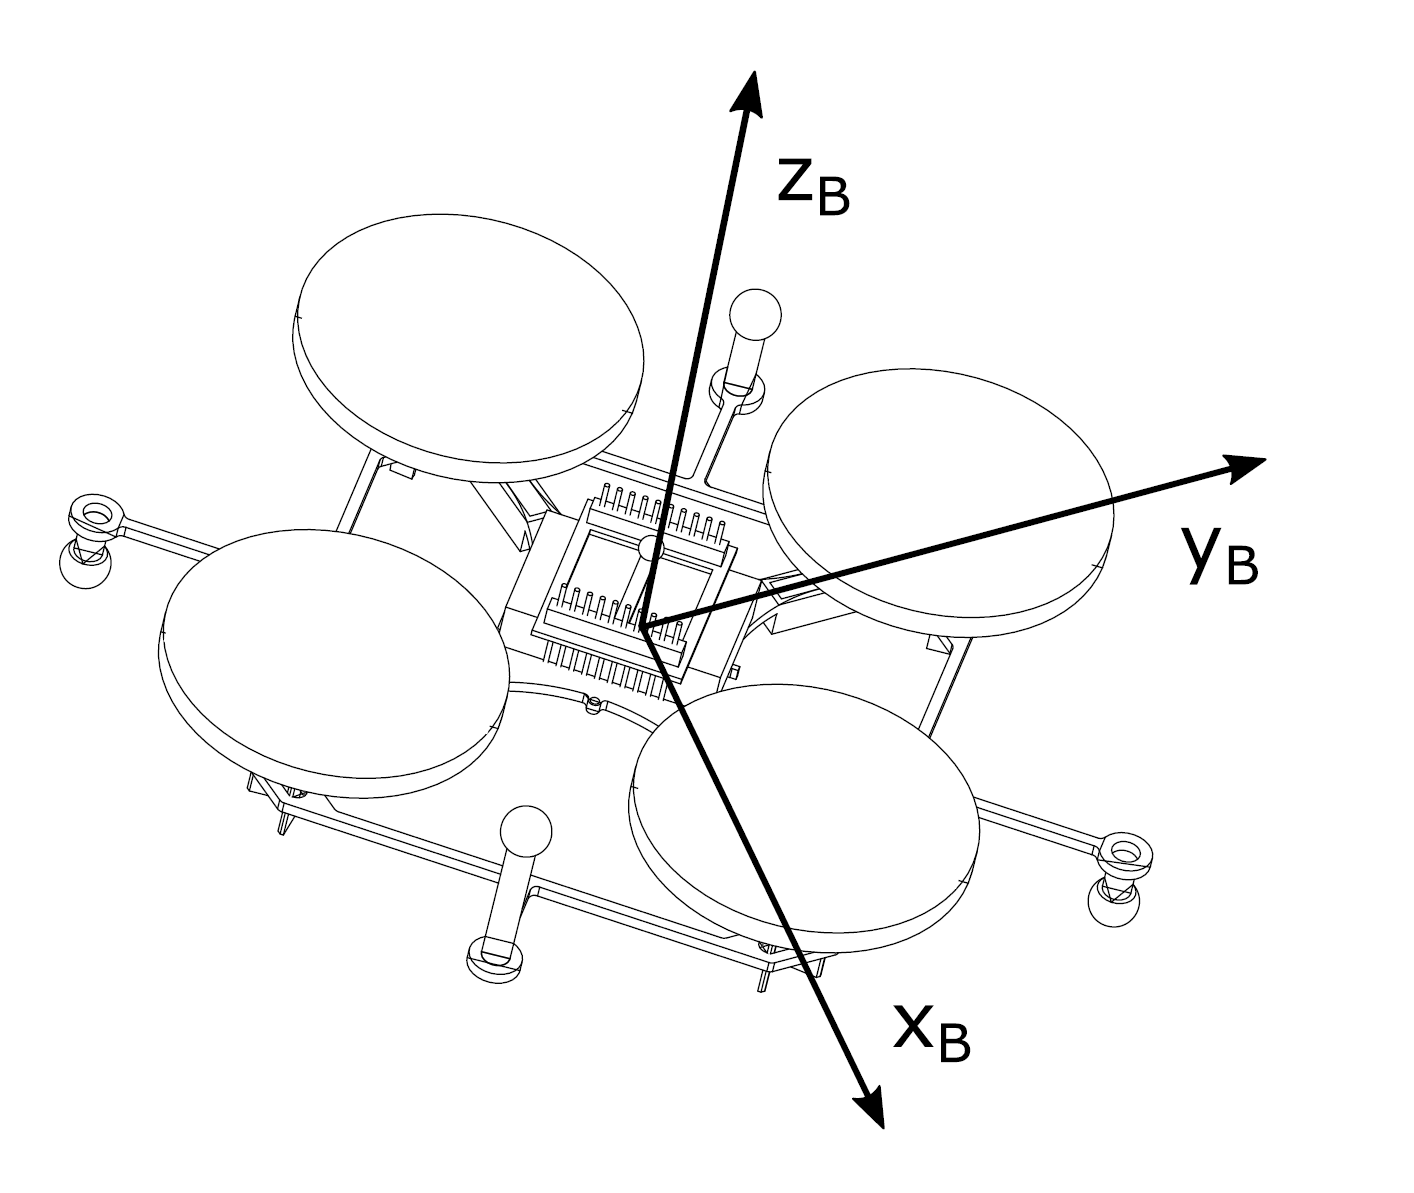
\includegraphics[width=0.9\linewidth]{img_crazyfly}
	\centering
	\caption{\label{fig: img_crazyfly}Model of the quadrotor used, the Crazyflie Nano
		Quadcopter, and the body frame used in the differentially flat
		model. $\boldsymbol{z_{B}}$ points in the same direction as propellers at all the time.}
\end{figure}
The model used in the study consists of a single floating rigid body and four
inputs. We define the inputs as the square of the angular velocities $\omega^2$ of the motors on the quadrotor. A spinning
propeller produces two forces on the quadrotor, namely lift
and drag. Those forces are directly proportional to $\omega^2$. Each
input $\omega_{i}^2$ can therefore be said to produce a certain linear
force $F_{i}$ on the center of mass as well as to create a moment $M_{i}$ according to\begin{equation} \label{eq: force_init}
F_{i} = k_{f}\omega_{i}^2,
\end{equation}\begin{equation} \label{eq: moment_init}
M_{i} = k_{m}\omega_{i}^2.
\end{equation}

We can then write the dynamics of the quadrotor:\begin{equation} \label{eq: dynamics_1}
m\ddot{r} = mg\boldsymbol{z_{w}} + (\sum_{i=1}^{4}F_{i})\boldsymbol{z_{b}},
\end{equation}\begin{equation} \label{eq: dynamics_2}
\boldsymbol{\dot{\omega}} = I_{}^{-1}(-\boldsymbol{\omega} \times I\boldsymbol{\omega} + W),
\end{equation}\begin{equation} \label{eq: dynamics_3}
W = \begin{bmatrix}
0 & k_{f}L & 0  & -k_{f}L \\ 
-k_{f}L & 0 & k_{f}L  &  0\\ 
k_m & -k_m & k_m & -k_m
\end{bmatrix}\begin{bmatrix}
\omega_{1}^2\\ 
\omega_{2}^2\\ 
\omega_{3}^2\\ 
\omega_{4}^2\\
\end{bmatrix},
\end{equation}where $m$ is the mass of the quadrotor, $\ddot{r}$ is the acceleration of its center of mass, $\boldsymbol{z_w}$ is a unit vector in the direction of gravity, $\boldsymbol{z_b}$ is a unit vector pointing in the same direction as the propellers (in the world frame), $I$ is the inertia matrix of the quadrotor, $L$ is the distance between each propeller and the center of mass of the quadrotor, and $\boldsymbol{\omega}$ is the angular velocity of the quadrotor in the body frame~\cite{richter2013polynomial}. 

We solve the problem of identifying the parameters of
this model with a two step approach. First, we directly or
semi-directly measure each parameter of the model with a
series of simple experiments. Second, we log flight data for a
series of maneuvers using a motion capture system, and use
an optimization-based algorithm to adjust those parameters. The $k_f$ parameter was identified by measuring the thrust
produced by the quadrotor placed upside-down on a scale and
fitting the corresponding parameter. The $k_m$ parameter can
be measured by slowly increasing a pair of opposite motors
(motors spinning in the same direction) and measuring the
resulting angular velocities using the on-board gyroscope. 

\section{Avoiding Obstacles}
The problem of obstacle avoidance is particularly chal-
lenging because the set of points outside a closed, bounded
obstacle is non-convex. As a result, we must generally add
non-convex constraints to an optimization in order to ensure
that our trajectory remains outside the set of obstacles. Such
constraints generally prevent us from finding guarantees of
completeness or global optimality in our program.~\cite{boyd2004convex}. We
can avoid some of the problems of non-convex constraints
by adding a discrete component to our optimization. If we model the non-convex set of obstacle-free states as the
union of finitely many convex regions, then we can perform
a mixed-integer convex optimization in which the integer
variables correspond to the assignment of trajectory seg-
ments to convex regions. This is not without consequences,
since even the addition of binary variables (that is, integer
variables constrained to take values of 0 or 1) turns linear
programming into mixed-{0, 1} linear programming, which
is known to be NP-complete.~\cite{karp2010reducibility}. However, excellent tools
for solving a variety of mixed-integer convex problems have
been developed in the past decade, and these tools can often
find globally optimal solutions very efficiently for mixed-
integer linear, quadratic, and conic problems~\cite{optimization2014gurobi,aps2014mosek,ilog2010cplex}. These tools also offer some anytime capability, since they can
be commanded to return a good feasible solution quickly or
to spend more time searching for a provably global optimum.

\par Earlier implementations of mixed-integer obstacle avoid-
ance have typically used the faces of the obstacles themselves
to define the convex safe regions. The requirement that a
point be outside all obstacles is converted to the requirement
that, for each obstacle, the point must be on the outside
of at least one face of that obstacle. For convex obstacles
these conditions are equivalent~\cite{mellinger2012mixed}. This approach has been successfully used to encode obstacle avoidance for UAVs as a
mixed integer linear program (MILP) by Schouwenaars~\cite{schouwenaars2001mixed}, Richards~\cite{richardsco}, Culligan~\cite{culligan2006online} and Hao~\cite{hao2005differential}. Mellinger et al.
add a quadratic cost function to turn the formulation into a
mixed-integer quadratic program (MIQP)~\cite{mellinger2012mixed}. However, this
approach requires separate integer variables for every face of
every obstacle, which causes the mixed-integer formulation
to become intractable with more than a handful of simple
obstacles.

Instead, IRIS, a greedy
tool for finding large convex regions of obstacle-free space is used here~\cite{deits2015computing}, to create a small number of convex regions to cover
all or part of the free space. These regions can be seeded
automatically based on heuristic methods or by an expert
human operator. We then need only one integer variable
for each region, rather than for each face of every obstacle.
We have previously demonstrated this approach for mixed-
integer footstep planning~\cite{deits2014footstep}, and it is also evident from the proofs shown in the following chapters that it
allows us to handle environments with tens or even hundreds
of obstacle faces.

\section{Safety of the Entire Trajectory}
Through the proposed approach, we have the ability to ensure that the
polynomial trajectory for the UAV is obstacle-free over its
entire length, rather than at a series of sample points. Existing
mixed-integer formulations have chosen only to enforce the
obstacle-avoidance constraint at a finite set of points~\cite{mellinger2012mixed,schouwenaars2001mixed,richards2002aircraft}. \begin{figure}[t]
	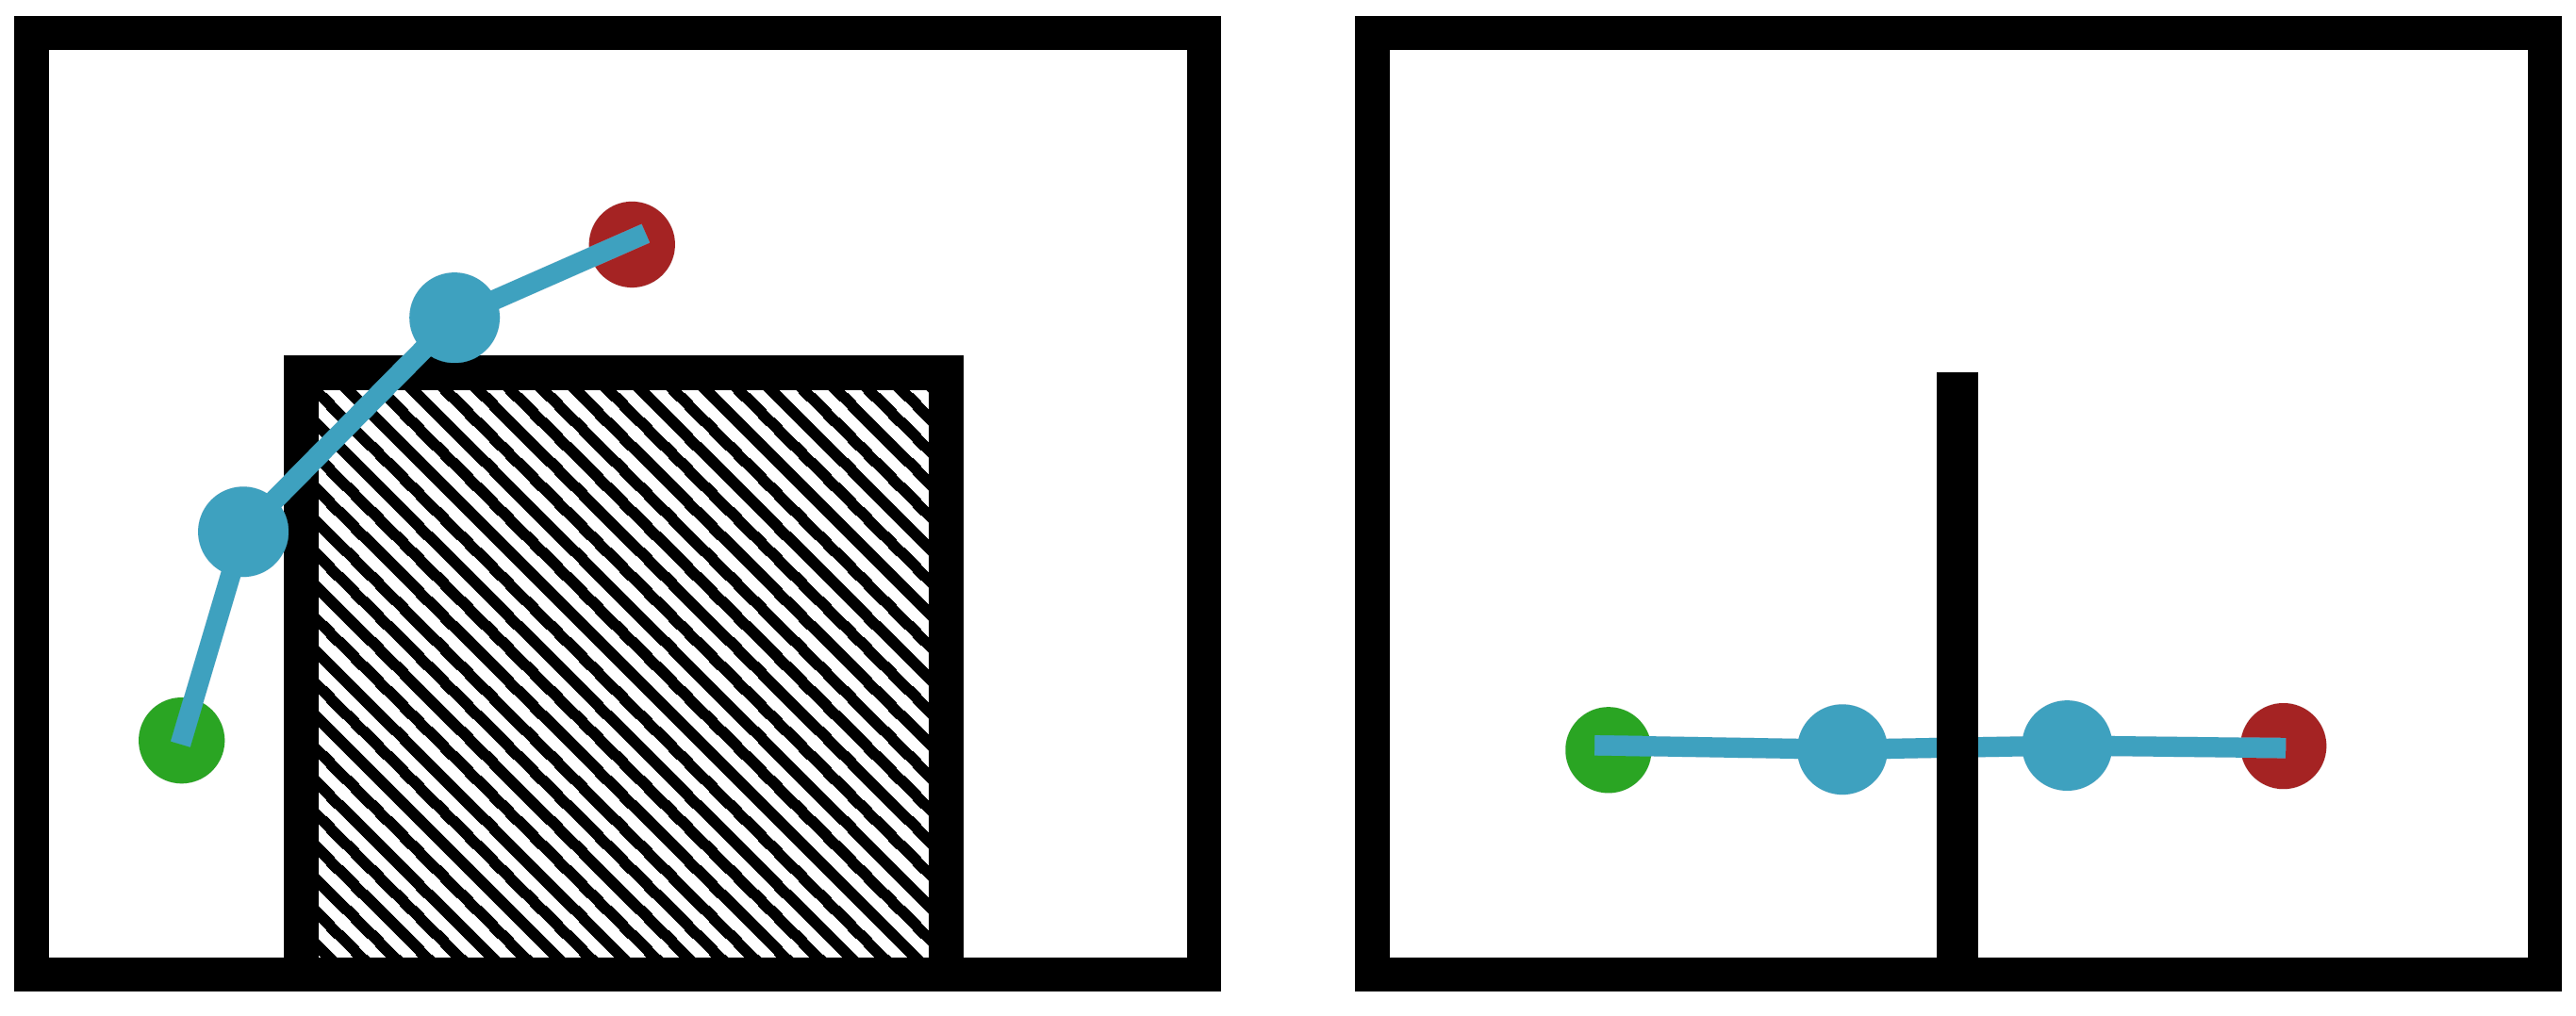
\includegraphics[width=0.9\linewidth]{fig_2}
	\centering
	\caption{\label{fig: cornercutting_1}A piecewise linear trajectory between two points, with obstacle
		avoidance enforced only at 4 points along each trajectory. The continuous
		trajectory through those points may cut corners or pass through thin
		obstacles.}
\end{figure}\begin{figure}[t]
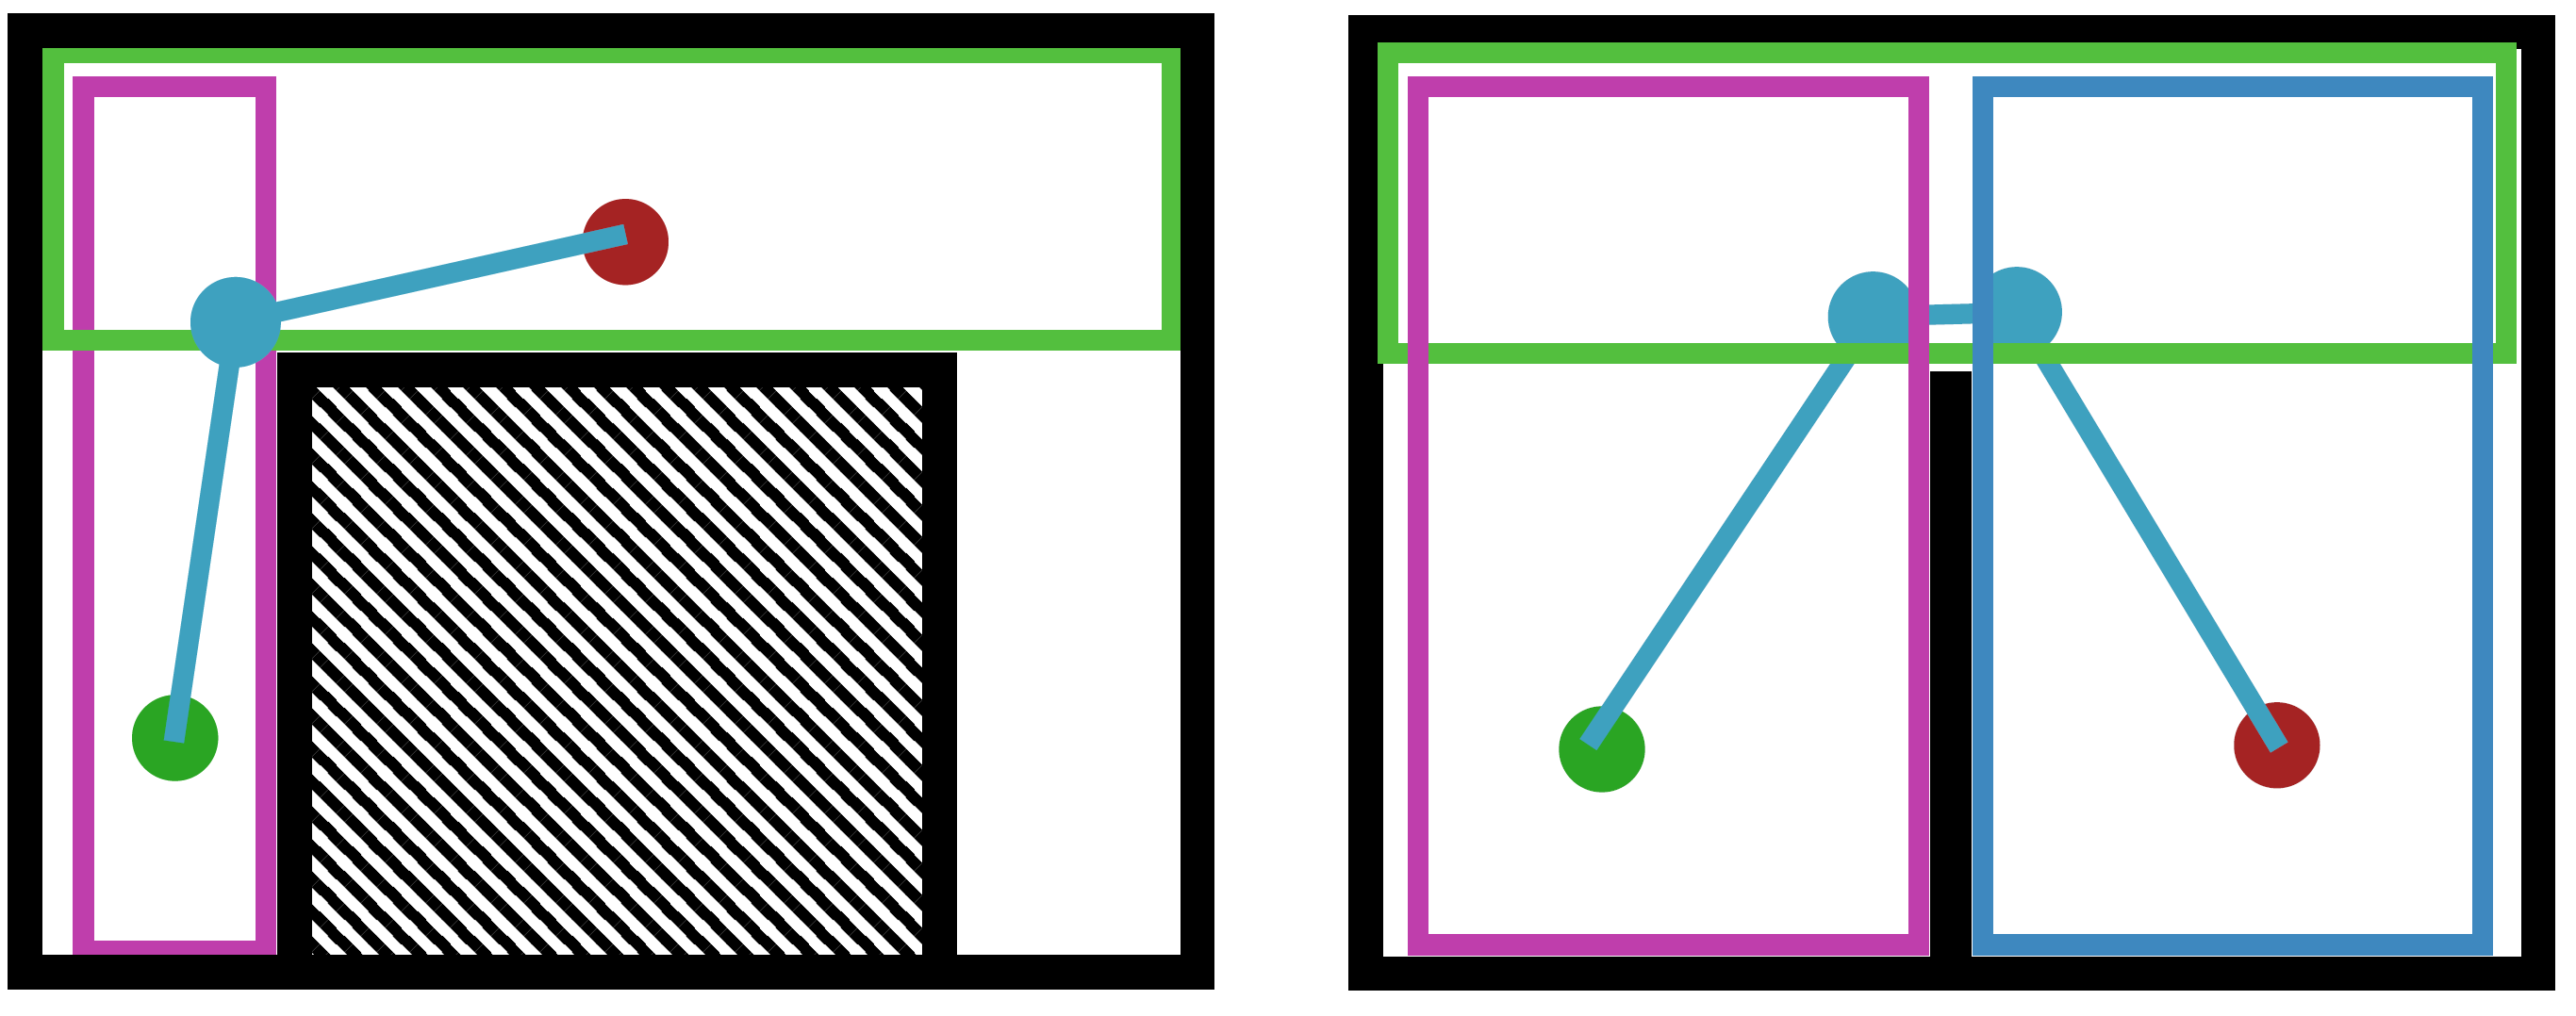
\includegraphics[width=0.9\linewidth]{fig_3}
\centering
\caption{\label{fig: cornercutting_2}A trajectory in which each linear segment is required to remain en-
	tirely within one of the convex obstacle-free regions indicated by the colored
	boxes. This requirement ensures that the entire trajectory is collision-free.}
\end{figure}This can result in the path between those sample
points cutting the corners of obstacles, or, more dangerously,
passing through very thin obstacles, as shown in Fig.~\ref{fig: cornercutting_1}. As noted by~\cite{bellingham2002coordination}, the severity of the corner cuts
can be reduced by increasing the number of sample points
and limiting the total distance between adjacent samples,
but this also increases the complexity of the optimization problem. Mellinger approaches this problem by requiring
that the bounding boxes of the UAV at adjacent sample points
must overlap~\cite{mellinger2012mixed}. This is sufficient to ensure that the UAV
never passes entirely through an obstacle, but it does not
necessarily prevent corner cutting. 

Representing the environment with convex safe regions
allows us to completely eliminate the cutting of corners. If
we treat the problem as one of assigning entire segments
of trajectories, rather than points, to the safe regions, then
we can create a fully collision-free trajectory. For piecewise
linear trajectories, this is simply a matter of ensuring that, for
each linear segment, both endpoints must be contained within
the same convex safe region, as shown in Fig.~\ref{fig: cornercutting_2}. This decision weakens our claim of optimality, since it requires the
breakpoints between trajectory segments to occur in the inter-
section of two convex regions, but it results in a formulation
that can be solved exactly with mixed-integer programming.
We enforce the constraint that each polynomial lie within a
convex region using a sums-of-squares (SOS) approach. In
this way, collision-free trajectories can be generated using
piecewise polynomials of arbitrary degree. Here we show
that, for trajectory segments defined by polynomials, we can
exactly enforce the constraint that each segment lies inside
a convex region by solving a small semi-definite program(SDP).


These polytopes, generated from IRIS must be given as an ordered union of only
pairwise adjacent sets, but the trajectories are guaranteed to
be contained within the polytopes by construction. Since the polytopes must be pairwise adjacent, they must be laid out
along a single path from start to goal by some other planning
procedure, and the resulting trajectories may not leave this
path. On the other hand, by performing our mixed-integer
optimization, we are able to explore arbitrarily connected
polytopes which may admit many different possible paths
through them.





 % Introduction
	
	\chapter{Technical Approach}

The proposed trajectory planning problem has three
components:\begin{enumerate}
	\item Generating convex safe regions
	\item Assigning trajectory segments to those convex regions and
	\item Optimizing the trajectories while ensuring that they remain
	fully within the safe regions.
\end{enumerate} Step (1) as a pre-
processing stage, then (2) and (3) are performed simultaneously in
a single mixed-integer convex optimization, which can be
solved to global optimality.

\section{Generating Convex Regions of Safe Space}

The user's ability to efficiently segment the space into convex
regions relies on our recent development of IRIS (Iterative
Regional Inflation by Semidefinite programming)~\cite{deits2015computing}. IRIS
alternates between two convex optimizations that (A) find a
set of hyperplanes which separate some ellipsoid from the
obstacles and (B) find the largest-volume ellipsoid within
those hyperplanes. Given an initial seed point in space,
around which the first ellipsoid is constructed, IRIS grows
the ellipsoid greedily at every iteration until it reaches a local
fixed point. The final set of separating hyperplanes forms a
(convex) polytope, which we take as our convex region of
obstacle-free space. Additional runs of IRIS with different
seed points produce additional obstacle-free regions.

Our initial applications of IRIS to the footstep planning
problem for walking robots relied on a human user to
choose the seed points for IRIS~\cite{deits2014footstep}. Human input was
valuable for that problem, since the choice of seed locations
allowed an expert operator to provide high-level input such
as which surfaces should be used for stepping. Manually
seeded regions are, of course, also possible in the case of an
aerial vehicle, and we expect that having an expert operator
choose the location of the seeds might be beneficial when
the environment is largely static and known beforehand.
However, this requirement is overly restrictive in the general
case.

\section{Searching over Assignments of Polynomials to Regions}

We encode the assignment of each polynomial piece of the
trajectory to a safe region using a matrix of binary integer variables ${H_{r,j}} \in \begin{Bmatrix}0,1 \end{Bmatrix}^{R \times N}$, where $R$ is the number of regions and $N$ is the number of polynomial trajectory pieces.
The polynomial trajectory pieces are labeled as $P_{j}(t)$ and the
convex regions as $\mathcal{G}_{r}$. Thus, we have:\begin{equation} \label{eq:implication}
{H_{r,j}} \Rightarrow {p_{j}}(t) \in \mathcal{G}_r \qquad \forall t \in [0,T_j]
\end{equation}

The range of $[0, 1]$ for time is chosen arbitrarily for simplicity in this
discussion, but any desired time span can be chosen when
constructing the problem. The actual time spent executing
each trajectory segment can also be adjusted as a post-
processing step by appropriately scaling the coefficients. 

Ensuring that polynomial $j$ is collision-free is expressed
with a linear constraint on $H$:\begin{equation} \label{eq:summation_Hrj}
\sum_{r=1}^{R}H_{r,j} = 1
\end{equation}
Note that the regions do overlap, so it is possible
for a polynomial to simultaneously exist within multiple
regions $\mathcal{G}_{r}$ . Such a case is allowed by the proposed formulation, since the implication in~\ref{eq:implication} is one-directional (so polynomial $P_j(t)$ being contained in $\mathcal{G}_r$ does not necessarily require that $H_{r,j} = 1$). We show in next section that the constraint $P_{j}(t) \in \mathcal{G}_{r} \forall t \in [0, 1]$ is convex, and we can use a standard big-M formulation~\cite{lofberg2004yalmip} to convert the implication in~\ref{eq:implication} to a linear
form. 

\section{Restricting a Polynomial to a Polytope}

The trajectories are represented in $n$ dimensions as piecewise
polynomials of degree $d$ in a single variable, $t$. Each segment
$j$ of the trajectory is parameterized by $d + 1$ vectors of
coefficients $C_{j,k} \in \mathbb{R}^n$  of a set of polynomial basis functions, $\Phi_{1}(t), ... , \Phi_{d+1}(t)$. For each segment $j$, the trajectory can be evaluated as\begin{equation} \label{eq:Pjt_eq3_deits}
P_{j}(t) = \sum_{k=1}^{d+1} C_{j,k} \Phi_{k} (t) \quad \quad t \in [0,1]
\end{equation} $R$ convex regions of safe space are restricted to be
polytopes, so for each region $r \in 1, . . . , R$, some
$A_r \in \mathbb{R}^{m \times n}$ and $b_r \in \mathbb{R}^{m}$ and the constraint that\begin{equation} \label{eq:eq4_deits}
A_{r}P_j(t) \leq b_r
\end{equation}if $H_{r,j}$ is set to 1. To ensure that the trajectory remains
entirely within the safe region,~\ref{eq:eq4_deits} must hold $\forall t \in [0, 1]$.  \begin{equation} \label{eq:eq5_deits}
A_{r}\sum_{k=1}^{d+1} C_{j,k} \Phi_k(t) \leq b_{r} \quad \quad \forall t \in [0,1]
\end{equation}
Eq.~\ref{eq:eq5_deits} consists of $m$ constraints of the form\begin{equation} \label{eq:eq6_deits}
a_{r,l}^{T}\sum_{k=1}^{d+1} C_{j,k} \Phi_k(t) \leq b_{r,l} \quad \quad \forall t \in [0,1]
\end{equation}where \begin{equation} \label{eq:eq7_deits}
A_r = \begin{bmatrix}a_{r,1}^{T}
\\ a_{r,2}^{T}
\\ .
\\ .
\\ .
\\ a_{r,m}^{T}
\end{bmatrix} \quad \text{and} \quad b = \begin{bmatrix}b_{r,1}
\\ b_{r,2}
\\ .
\\ .
\\ .
\\ b_{r,m}
\end{bmatrix}
\end{equation}

Redistributing the terms in~\ref{eq:eq6_deits} to get\begin{equation} \label{eq:eq8_deits}
\sum_{k=1}^{d+1} (a_{r,l}^{T}C_{j,k}) \Phi_{k}(t) \leq b_{r,l} \quad \quad \forall t \in [0,1] 
\end{equation} and thus \begin{equation} \label{eq:eq9_deits}
q(t) := b_{r,l} - \sum_{k=1}^{d+1} (a_{r,l}^{T}C_{j,k}) \Phi_{k}(t) \geq 0 \quad \quad \forall t \in [0,1] 
\end{equation}
The condition that $q(t) \geq 0 \quad \forall t \in [0, 1]$ holds if and only if
$q(t)$ can be written as	\begin{align} \label{eq:eq10_deits}
q(t) &= t\sigma_{1}(t) + (1-t)\sigma_{2}(t) \quad \quad \text{if $d$ is odd} \nonumber\\  &= \sigma_{1}(t) + t(1-t)\sigma_{2}(t) \quad \quad \text{if $d$ is even}
\end{align}
where the most important condition for viability of~\ref{eq:eq10_deits} is: 
$\sigma_{1}(t), \sigma_{2}(t) \text{ are sums of squares}$, where $\sigma_{1}(t)$ and $\sigma_{2}(t)$ are polynomials of degree $d -$1 if
$d$ is odd and of degree $d$ and $d -$2 if $d$ is even~\cite{parrilo2006sums}. The condition that $\sigma_{1}(t), \sigma_{2}(t) \text{ are sums of squares}$ requires that
each can be decomposed into a sum of squared terms, which
is a necessary and sufficient condition for non-negativity for
polynomials of a single variable~\cite{parrilo2006sums}. The coefficients of
the polynomials $\sigma_{1}$ and $\sigma_{2}$ are additional decision variables
in our optimization, subject to linear constraints to enforce~\ref{eq:eq10_deits}.  The sum-of-squares constraints can be rep-
resented in general with a semidefinite program~\cite{powers1998algorithm}. The problem of assigning the trajectories to safe regions is thus
a mixed-integer semidefinite program (MISDP). This class
of problems can be solved to global optimality using, for
example, the Yalmip branch-and-bound solver or with a semidefinite programming solver like Mosek~\cite{aps2014mosek}. Successful validation for the above formulation is applied to polynomials of degree 1, 3 and 5. For polynomials of degree 7 and higher, due to numerical difficulties
which often prevented Mosek from solving the semidefinite
program, more numerically stable exact reductions for lower degree polynomials is proposed.

For polynomials of degree 1, $\sigma_{1}$ and $\sigma_{2}$ are constants, and
the condition of being the sums of squares reduces to linear constraints\begin{equation} \label{eq:eq12_deits}
\sigma_{1} \geq 0, \sigma_{2} \geq 0,
\end{equation} which reduces the problem to a mixed-integer quadratic
program (MIQP), given our quadratic objective function.
If the polynomials are of degree 3, then $\sigma_{i}(t)$ is a quadratic
polynomial:\begin{equation} \label{eq:eq13_deits}
\sigma_{i}(t) = \beta_{1} + \beta_{2}(t) + \beta_{3}(t)^2.
\end{equation}
Using the standard sum-of-squares approach, we rewrite
$\sigma_{i}(t)$ as\begin{equation} \label{eq:eq14_deits}
\sigma_{i}(t) = \begin{bmatrix}1
& t
\end{bmatrix} \begin{bmatrix}\beta_{1}
& \beta_{2}/2\\ \beta_{2}/2 
& \beta_{3}
\end{bmatrix} \begin{bmatrix}1
\\ t
\end{bmatrix}
\end{equation}
The condition that $\sigma(t)$ is SOS is equivalent to the matrix
of coefficients in~\ref{eq:eq14_deits} being positive semi-definite:\begin{equation} \label{eq:eq15_deits}
\begin{bmatrix}\beta_{1}
& \beta_{2}/2\\ \beta_{2}/2 
& \beta_{3}
\end{bmatrix} \geq 0,
\end{equation}which is in turn equivalent to the following rotated second-
order cone constraint:
\begin{equation} \label{eq:eq16_deits}
\beta_{2}^2 - 4\beta_{1}\beta_{3} \leq 0
\end{equation}\begin{equation} \label{eq:eq17_deits}
\beta_{1}, \beta_{3} \geq 0
\end{equation}Thus the problem of assigning degree-3 poly-
nomials to convex regions as a mixed-integer second-order
cone problem (MISOCP) can be solved effectively
with Mosek~\cite{aps2014mosek}.

\section{Choosing Objective Function}
If $P_{j}(t)$ is of degree $d \geq$ 4, then according to Mellinger et al. who relate the snap (that is, the fourth derivative
of position) to the control inputs of a quadrotor, and thus
an objective of the form: \begin{equation} \label{eq:eq18_deits}
\text{minimize} \quad \sum_{j=1}^{N} \int_{0}^{1}\begin{Vmatrix}\frac{\mathrm{d}^4 }{\mathrm{d} t^4}
P_{j}(t) 
\end{Vmatrix}{\mathrm{d}t}
\end{equation}
If $P_{j}(t)$ is of degree $d \geq$ 4 then we may do likewise, resulting
in a convex quadratic objective on the coefficients of the $P_{j}$.
Demonstrating this objective function in operation with $5^{th}$ degree polynomials in Fig.~\ref{fig: figs-4a} and~\ref{fig: figs-4b}.

However, to reduce our problem to a MISOCP and improve the numerical stability of the solver, is is found that it is beneficial to restrict ourselves to $3^{rd}$-degree polynomials and thus piecewise constant jerk. Our objective is:
\begin{equation} \label{eq:eq19_deits}
\text{minimize} \quad \sum_{j=1}^{N} \int_{0}^{1}\begin{Vmatrix}\frac{\mathrm{d}^3 }{\mathrm{d} t^3}
P_{j}(t) 
\end{Vmatrix}{\mathrm{d}t}
\end{equation}which is likewise convex and quadratic in the coefficients
of the $P_j$ .Linear constraints are added on the position,
velocity, and acceleration of each trajectory piece to ensure
that they are continuous from one polynomial piece to the
next. Additional linear equality constraints require that the
position, velocity, and acceleration of the beginning of the
first trajectory piece and the end of the last piece match our
desired initial and final states, thereby giving a perfect smooth trajectory.
\begin{figure}[t]
	\hfill
	\subfigure[]{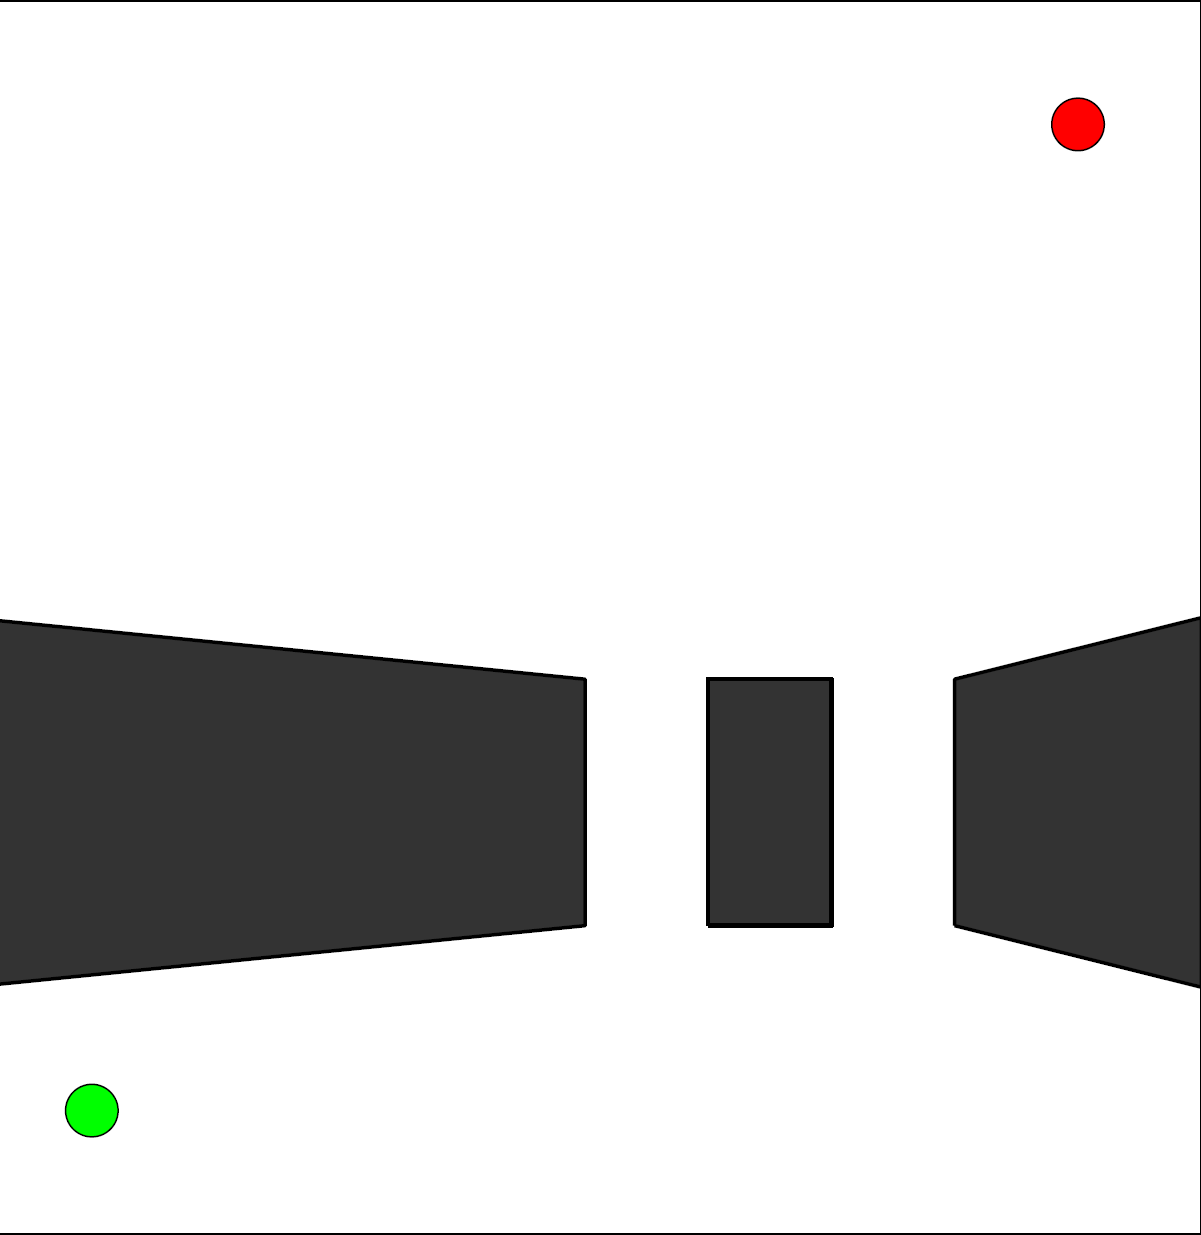
\includegraphics[width=0.48\linewidth]{4-a}}
	\hfill
	\subfigure[]{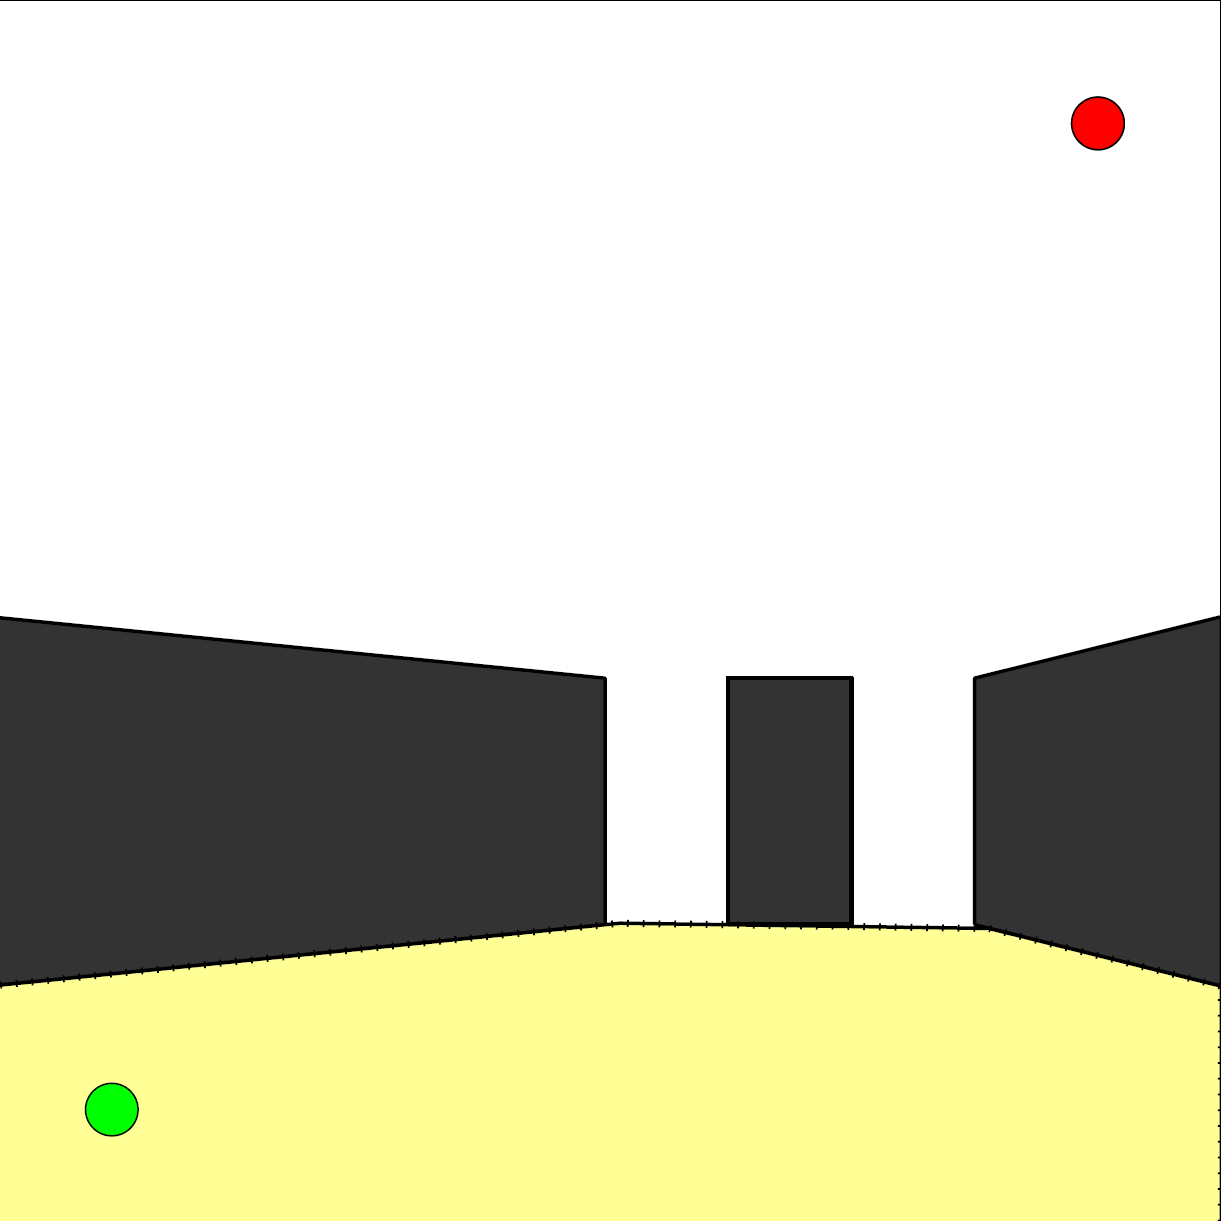
\includegraphics[width=0.48\linewidth]{4-b}}
	\hfill
	\subfigure[]{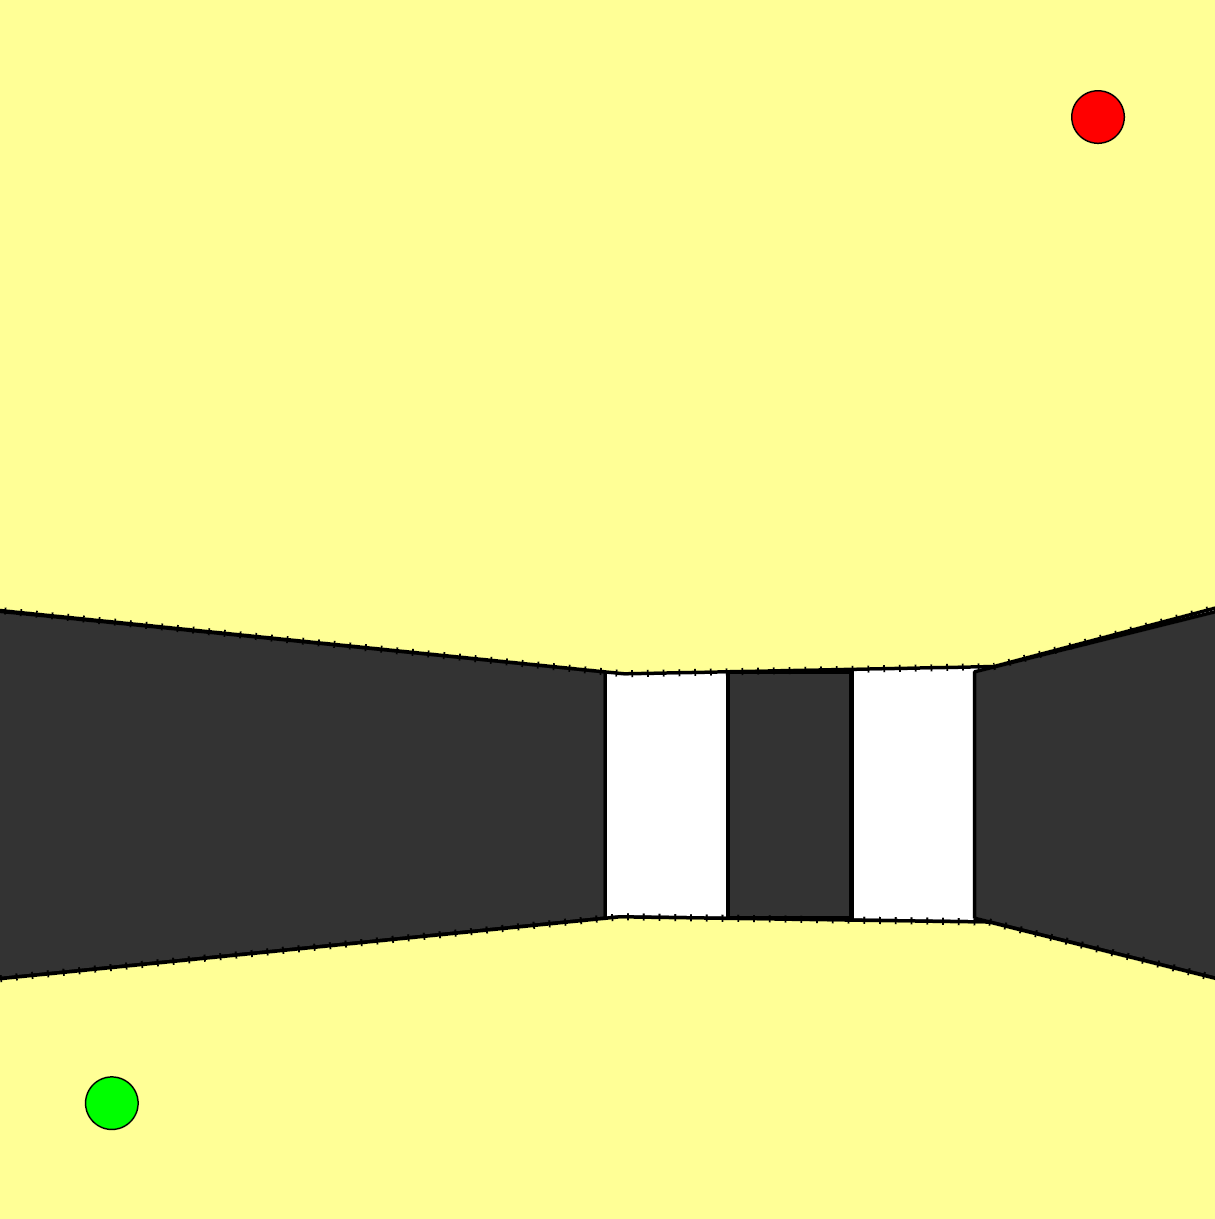
\includegraphics[width=0.48\linewidth]{4-c}}
	\hfill
	\subfigure[]{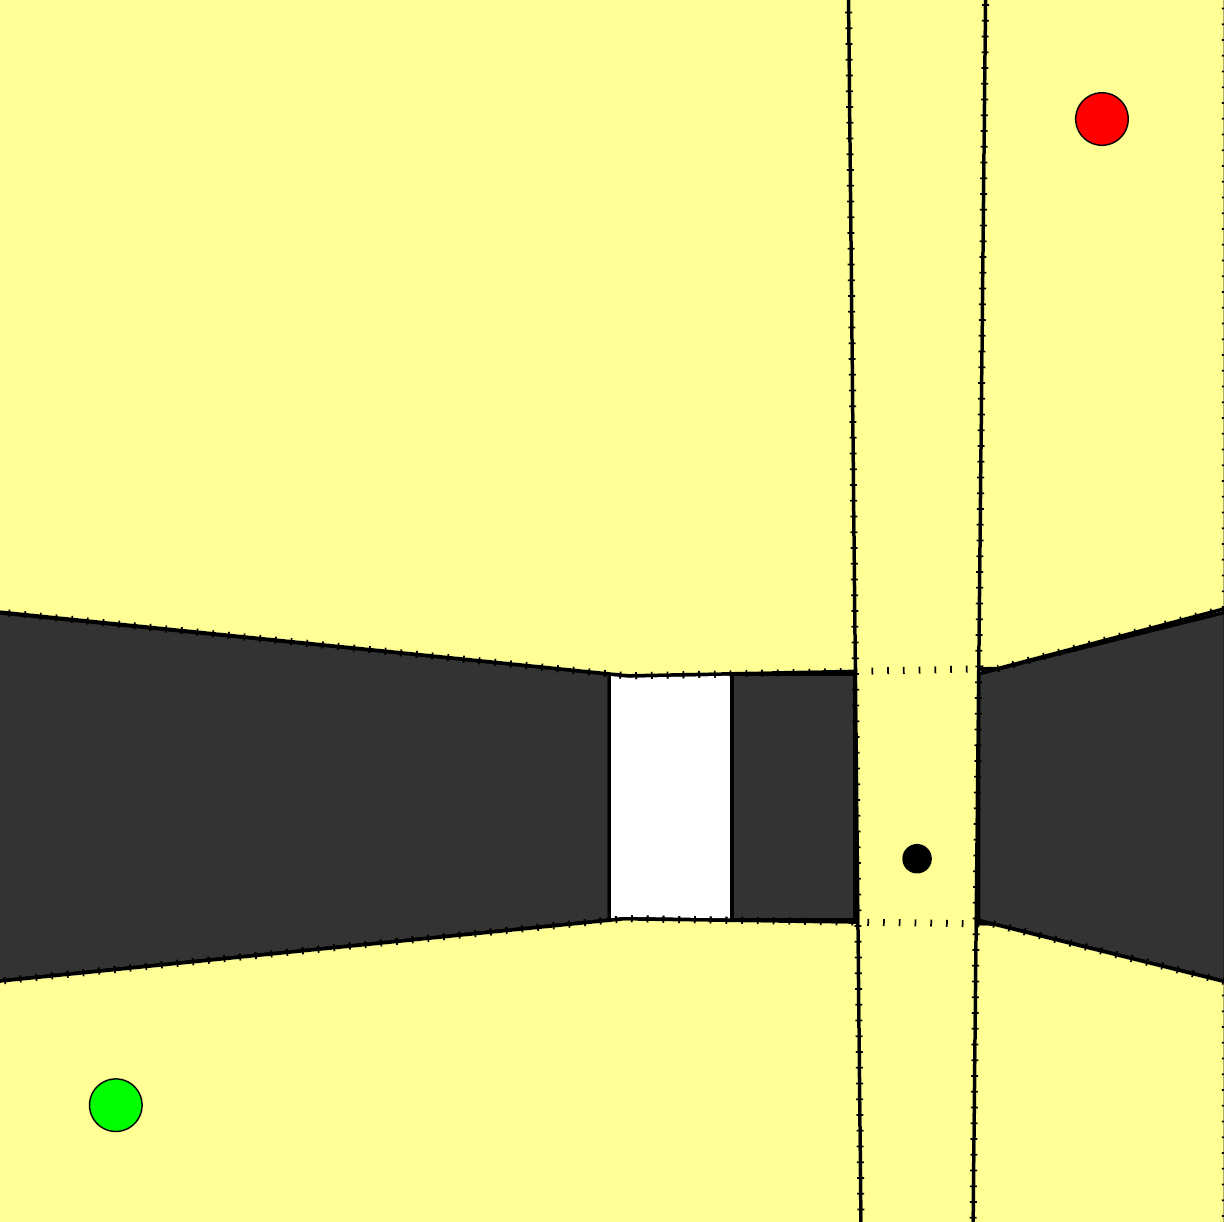
\includegraphics[width=0.48\linewidth]{4-d}}
	\hfill
	\caption{\label{fig: figs-4a}Solving a simple environment with IRIS regions. A random environment is constructed with obstacles and a start and goal pose (a), then generate IRIS regions around the start (b) and goal (c). Next, a point is identified far from the existing set of obstacles and IRIS regions and a new region is generated from the seed point there (d)}
\end{figure}
\begin{figure}[t]
	\hfill
	\subfigure[]{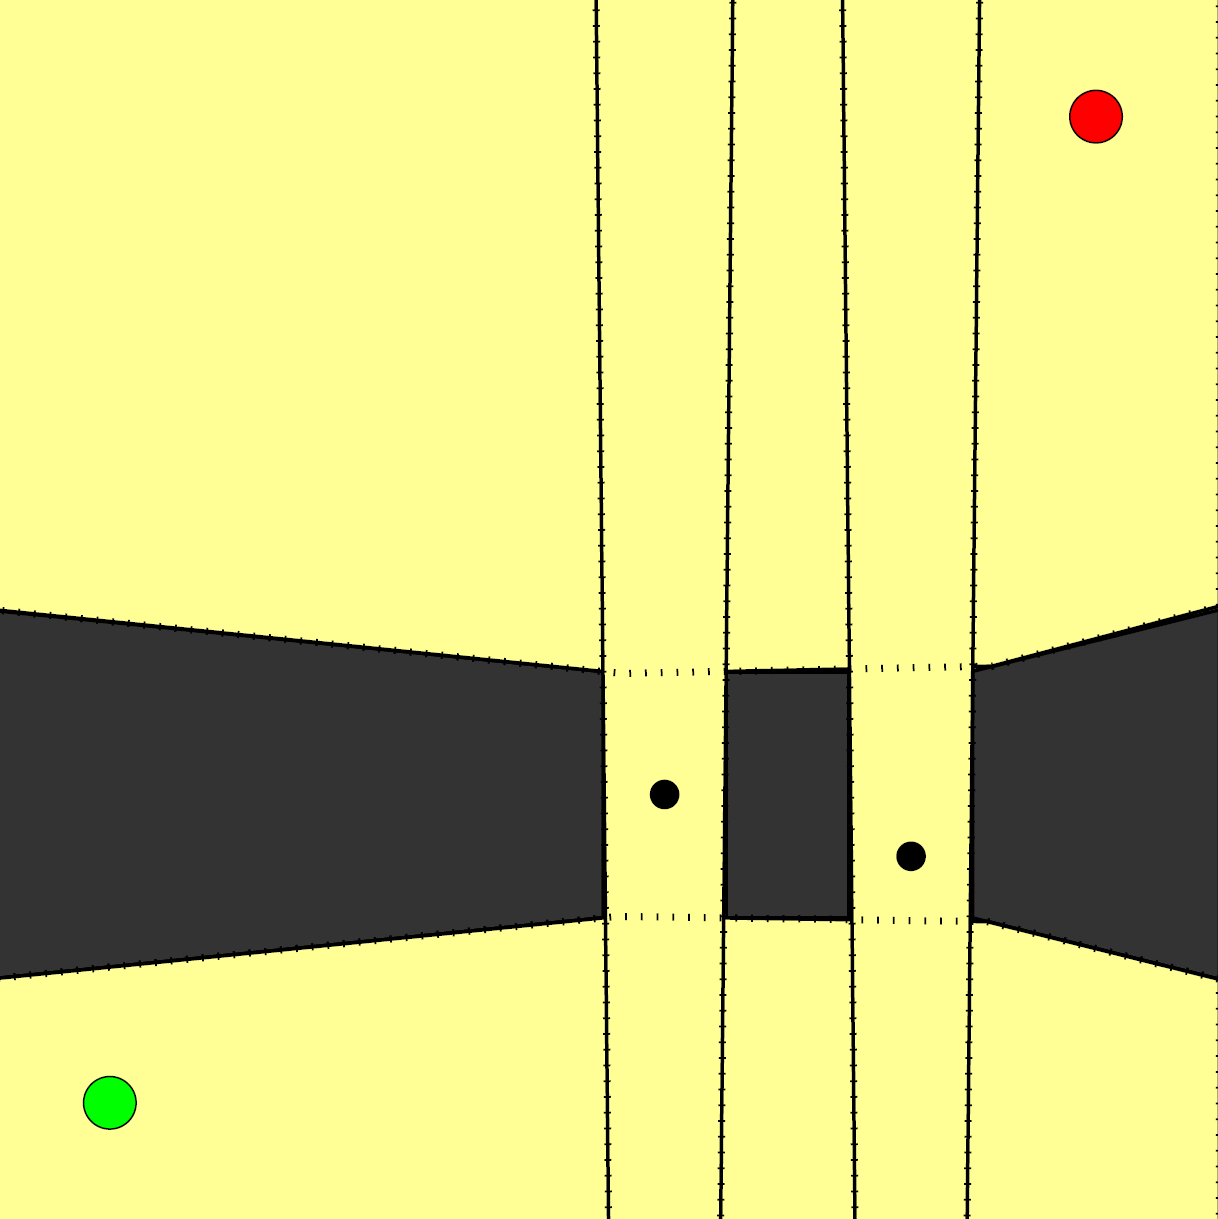
\includegraphics[width=0.48\linewidth]{4-e}}
	\hfill
	\subfigure[]{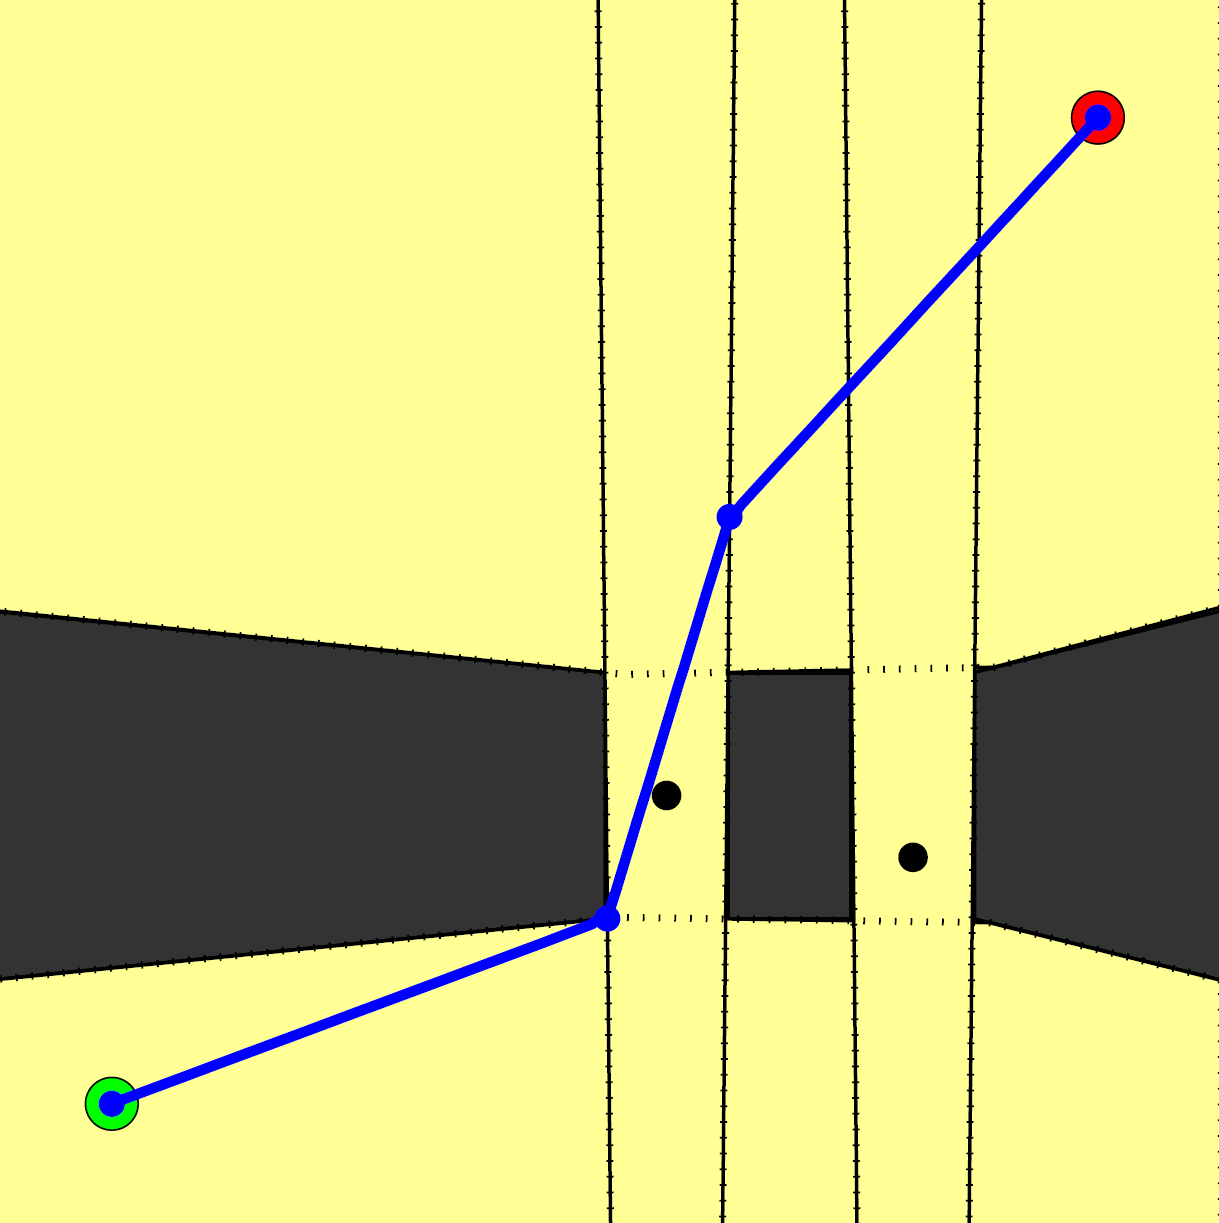
\includegraphics[width=0.48\linewidth]{4-f}}
	\hfill
	\subfigure[]{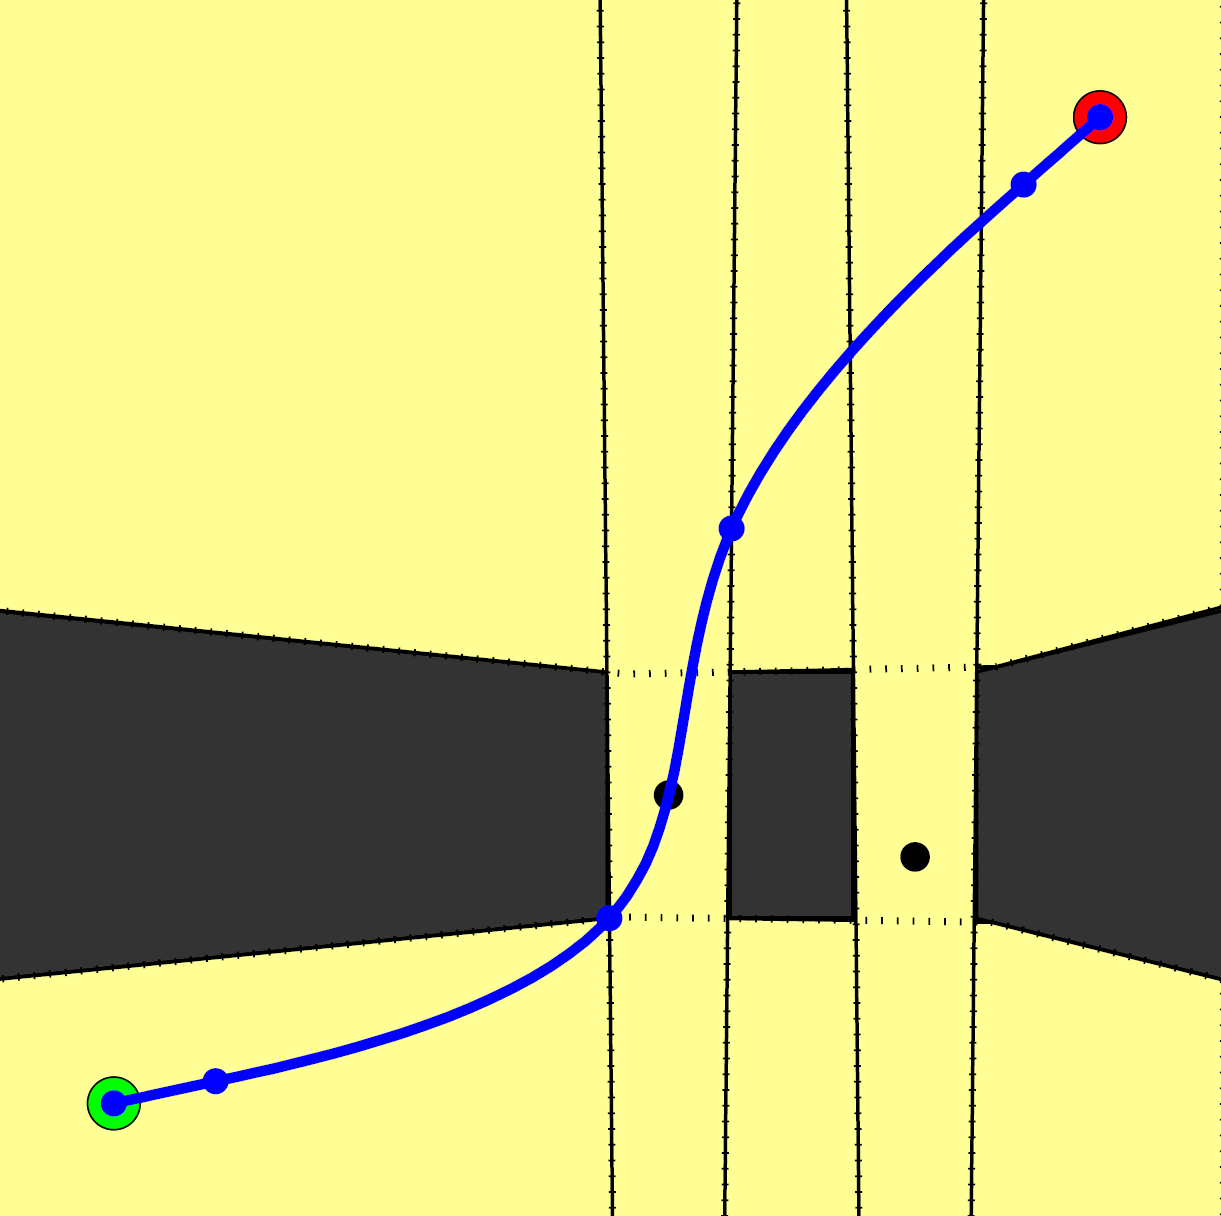
\includegraphics[width=0.48\linewidth]{4-g}}
	\hfill
	\subfigure[]{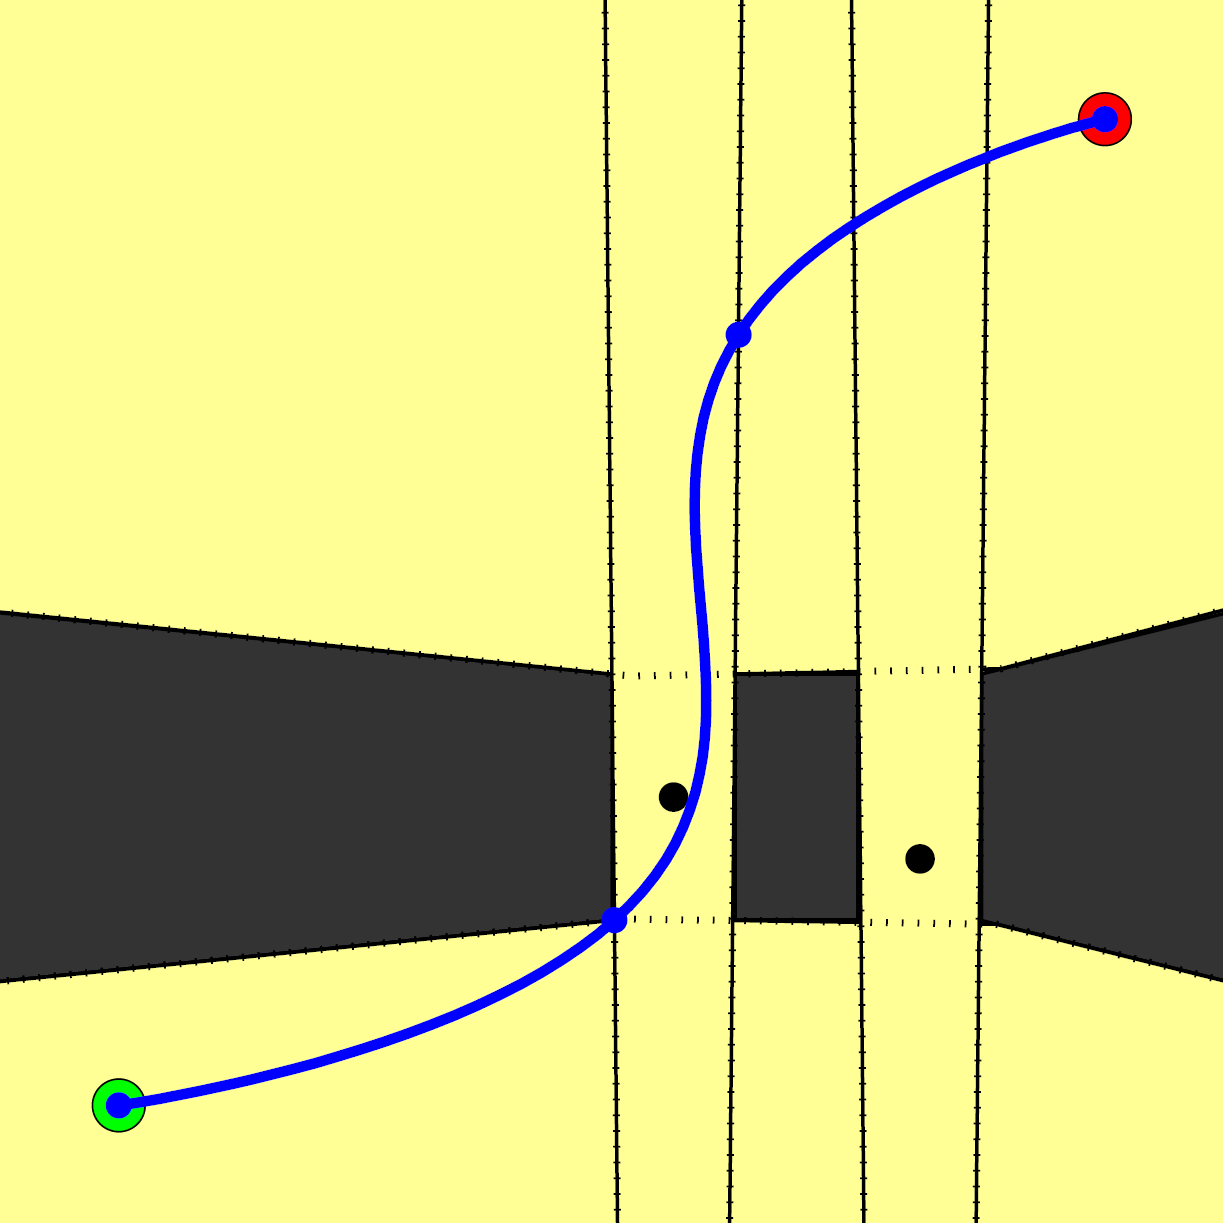
\includegraphics[width=0.48\linewidth]{4-h}}
	\hfill
	
	
	\caption{\label{fig: figs-4b}The above process through which we obtained (d) is repeated until we have 4 regions (e). Finally, we solve for trajectories of $1^{st}$-degree polynomials minimizing squared velocity in 0.1s (f), $3^{rd}$-degree polynomials minimizing squared jerk in 0.3s (g), and
		$5^{th}$-degree polynomials minimizing squared snap in 1.0s (h). All trajectories lie entirely within the convex regions shown.}
\end{figure}



\section{Handling Lower-Degree Trajectories}
Even if the mixed-integer optimization is done over the numerically easier degree $3$ polynomials, we can post-process the resulting trajectories in order to successfully use the differential flatness of the system to derive the full state and input. A piecewise degree-$3$ trajectory has a piecewise constant $3^{rd}$ derivative. It thus has delta functions for its $4^{th}$ derivative, which Mellinger relates directly to the rotor thrusts of the
UAV~\cite{mellinger2011minimum}. Since this is clearly undesirable, according the proposed approach we proceeded as follows: First, we ran the MISOCP to optimize our degree-$3$ polynomials and assign them to convex safe regions. Next, we fixed the resulting assignment of trajectories to safe regions and then re-ran the optimization for polynomials of degree
$5$ or higher while minimizing the squared norm of the snap. Since all of the integer variables are fixed, we no longer have a mixed-integer problem but instead a single semidefinite program, which can be solved very efficiently. 

\section{Complete Formulation}

Our optimization problem can be written as follows for a
trajectory of $N$ piecewise $3^{rd}$-degree polynomials:

	
\begin{equation}  \label{eq:eq20_deits}
\min_{P,H,\sigma} \quad  \sum_{j=1}^{N} \begin{Vmatrix}\frac{\mathrm{d}^3 }{\mathrm{d} t^3}
P_{j}(t) 
\end{Vmatrix}
\end{equation}subject to:


\[
\begin{array}{@{}l@{}} 
P_{1}(0) = {x_{0}}, \quad {P_{N}}(1) = {x_{f}}, \quad  {P_{j}}(1) = {P_{j+1}}(0) \\

{\dot{P_1}}(0) = {\dot{x_0}}, \quad {\dot{P_N}}(1) = c{\dot{x_f}}, \quad {\dot{P_j}}(1) = {\dot{P}_{j+1}}(0) \\

{\ddot{P_1}}(0) = {\ddot{x_0}}, \quad {\ddot{P_N}}(1) = {\ddot{x_f}}, \quad {\ddot{P_j}}(1) = {\ddot{P}_{j+1}}(0)

\end{array}
\]

\begin{equation}
	\forall j \in \begin{Bmatrix}1,
	&.  &.  &. & ,N 
	\end{Bmatrix}
\end{equation}

where $\sigma_{l,j,1}(t), \sigma_{l,j,2}(t) $ are sums of squares

	\[
	\begin{array}{@{}l@{}} 
	{H_{r,j}} \implies\\ \quad {b_{r,m}} - {A_{r,m}^{T}}{p_{j}}(t) = t{\sigma_{j,m,1}}(t) + (T_j - t){\sigma_{j,m,2}}(t)  \\ 
	
	\end{array}
	\]


\[
\begin{array}{@{}l@{}} 
\sum_{r=1}^{R}{H_{r,j}} = 1 \quad \forall j \in {1, ..., N}  \\ 
\end{array}
\]
	\begin{equation}  \label{eq:eq24_deits}
 {H_{r,j}} \in {0,1}
	\end{equation}
	
	where ${x_{0}}$ , $\dot{x_0}$ , $\ddot{x_0}$ are the initial position, velocity, and 	acceleration of the vehicle and ${x_{f}}$ , $\dot{x_f}$ , $\ddot{x_f}$ are the final values. All of the above conditions are linear constraints on the coefficients $C$ and $\beta$ and the matrix $H$, except the condition that $\sigma_1$ and $\sigma_2$ are sums of squares, which is a rotated second-order cone constraint.	 
 % Technical Approach
	
	\chapter{Conclusion}

We studied a new method for optimal trajectory planning around obstacles which ensures that the entire path is collision-free, rather than enforcing obstacle avoidance only at a set of sample points. This method is formulated
as a mixed-integer convex program and can be directly used with the mixed-integer obstacle avoidance approach which is already common in the field. Performance of our approach can be significantly improved by pre-computing convex regions of safe space with IRIS, a tool for greedy convex
segmentation, which can allow us to solve for trajectories even in very cluttered environments.

\section{Limitations}

By requiring that each polynomial trajectory piece lie entirely within one convex safe region, we disallow trajectories which may not intersect the obstacles but which pass through several safe regions. Our claims of global optimality are also limited to trajectories which obey this restriction.
This problem can be alleviated by increasing the number of trajectory segments so that each segment can be assigned to a single safe region, but doing so increases the complexity of the mixed-integer program. Successful trajectory generation is also dependent on the particular set of convex regions which are generated. In some environments, automatically finding regions at points far from the obstacles was sufficient, but as the
environment becomes more complex, we may require a more intelligent method of selecting the seed points at which the IRIS algorithm begins. Input from a human operator can be extremely helpful, a human operator indicated the interiors of the window and doorway as salient points at which to
generate convex regions, which allowed a feasible trajectory to be found with less time spent blindly searching for good
region locations.


Finally, in order to ensure a smooth control input, we may
wish to constrain the derivatives of the snap of the trajectory,
which will require polynomials of degree $5$ or higher. This
will require a more careful approach to ensure the numerical
stability of the mixed-integer semidefinite program. We are
not yet able to reliably solve these high-order problems
using Mosek without encountering numerical difficulties. The choice of basis functions $\Phi$ in Eq.~\ref{eq:Pjt_eq3_deits} is
likely to be a significant factor in the numerical stability
of the solver~\cite{mellinger2012mixed}. 

\section{Future Work}

In the future, intention to explore additional constraints
and objectives, such as waypoints in space which must be
visited en route from the start to the goal. Plans to study
investigate more effective heuristics for choosing the seed
points for the convex safe regions, including seeding regions
based on the results of a sample-based motion planner like 
RRT. Finally, we plan to study these trajectories into the real
world with their stabilization and execution on hardware. % Conclusion
	
	%\input{Chapters/Chapter4} % Experiment 1
	
	%\input{Chapters/Chapter5} % Experiment 2
	
	%\input{Chapters/Chapter6} % Results and Discussion
	
	%\input{Chapters/Chapter7} % Conclusion
	
	%% ----------------------------------------------------------------
	% Now begin the Appendices, including them as separate files
	
	\addtocontents{toc}{\vspace{2em}} % Add a gap in the Contents, for aesthetics
	
	\appendix % Cue to tell LaTeX that the following 'chapters' are Appendices
	
	\chapter{An Appendix}

Add appendices here	% Appendix Title
	
	%\input{Appendices/AppendixB} % Appendix Title
	
	%\input{Appendices/AppendixC} % Appendix Title
	
	\addtocontents{toc}{\vspace{2em}}  % Add a gap in the Contents, for aesthetics
	\backmatter
	
	%% ----------------------------------------------------------------
	\label{Bibliography}
	\lhead{\emph{Bibliography}}  % Change the left side page header to "Bibliography"
	\bibliographystyle{unsrtnat}  % Use the "unsrtnat" BibTeX style for formatting the Bibliography
	\bibliography{Bibliography}  % The references (bibliography) information are stored in the file named "Bibliography.bib"
	
\end{document}  % The End
%% ----------------------------------------------------------------